\documentclass{article}
\usepackage{amssymb, amsmath, graphicx}
\usepackage[margin=0.5in]{geometry}

\begin{document}

\title{Neural Turing Machines}
\author{Piyush Patil}
\maketitle

Neural networks have enjoyed considerable success in practice, and when they make use of non-linear activation functions such as squashing functions, they've been shown to conform to a range of universal approximation theorems, most notably for arbitrary measurable functions, and are Turing complete. Of course, Turing completeness is a theoretical ideal which requires access to virtually infinite, and a neural net that can in principle do anything a desktop computer can but which in practice requires enormous amounts of memory, prolonged periods of training time, and intractable amounts of data to train isn't useful in practice. Recurrent neural networks, or RNNs, have shown considerable improvement and perform very well on data similar to time series. The key to the success of certain RNNs, such as LSTMs, is their ability to employ feedback loops with the capacity to store information over time, analogous to the mammalian working memory. Neural turing machines, or NTMs, also seek to emulate working memory, but do so through a large space of addressable memory, rather than feedback loops, similar to Turing machines' use of an infinite tape of addressable memory, hence the name.
The motivation here is to separate computation from memory, rather than have both implicitly represented in a weight matrix as in conventional neural nets. The result is a sort of computer that loosely follows the von Neumann architecture, with an RNN acting as a sort of CPU, accessing a large memory bank of cells in a differentiable way. This allows the computer to learn different programs when faced with a problem, and actually come up with its own implementation of an algorithm to solve the problem. It seems like we go to great lengths to ensure that the entire model is, end-to-end, differentiable, but this is critically important because it allows us to train the model only with gradient descent. 

\section{Architecture}
NTMs consist of a simple RNN network, called the \textit{controller}, and a large real matrix, called with \textit{memory bank}. As usual, the controller network receives input vectors and produces output vectors, but it may read from and write to the memory bank in parallel upon receiving the input vector, allowing the stored memory to influence the output. We refer to the read and write operations as occuring through a \textit{read head} and a \textit{write head}, respectively. The read head outputs a read vector representing the accessed data, and doesn't alter the memory bank at all; the write head doens't output anything but alters the state of the memory bank. In contrast to the conventional model of computer memory as a large array or tape of cells which can be individually written to, we define our read and write heads in a global fashion, interacting with the whole memory matrix at once. This is required to ensure differentiability throughout the architecture, but forces the architecture to rely on "fuzzy" reading and writing. Of course, we rarely want to access or write to the entire memory bank at once, and much like a regular computer, we'll most often be updating or reading from specific cells or blocks of cells. To integrate this kind of block or local access in a fuzzy global operator, we need some kind of \textit{attention model}, ie a continuous (differentiable in fact) mechanism which allows the controller to read and write selectively to specific cells while leaving the remaining cells more or less untouched. Let's take a look at how we can implement one such attention model.

\subsection{Reading}
Define $ M^t \in \mathbb{R}^{n \times m} $ denote our memory bank at time $ t $, which we structure as $ n $ memory cells, each consisting of a real vector in $ \mathbb{R}^m $. To implement fuzzy differentiable reading from $ M^t $, the read head maintains a (normalized) weighting $ w^t \in \mathbb{R}^n $ across the memory bank, so that we can define a read operation to output a \textit{read vector} $ r^t \in \mathbb{R}^m $ given by
$$ r^t = \sum_{i = 1}^n w_i^t M_i^t $$
Notice that although the read vector is the result of a global operation, as we mentioned above, the use of a weighting across the memory bank allows us to attentionally focus on certain memory locations, assigning irrelevant memory locations low weight and relevant ones high weight. Clearly, $ r^t $ is totally differentiable.

\subsection{Writing}
We define the write head similarly to the read head, with a global operation across the entire memory bank. Because writing may require making use of existing memory locations rather than simply overwriting them, we break the write operation into a pipeline of two sub-operations - first, an \textit{erase} operation, followed by an \textit{add} operation (inspired by the input and forget gates in LSTMs). As with the read head, the write head maintains a (normalized) weighting $ w^t \in \mathbb{R}^n $, but also maintains an erase vector $ e^t \in [0, 1]^m $. We restrict the range of the erase vector to the unit box to accomodate the following definition of an erase operation.
$$ \forall i \in \{ 1, \cdots, n \}: M_i^t \gets M^{t - 1}_i \circ (\mathbf{1} - w_i^t e^t) $$
where $ \circ $ denotes the Hadamard, or element-wise, product and $ \mathbf{1} $ is the vector consisting of all 1's. Thus, the larger a given entry of the erase vector is, the more the corresponding entry in the memory bank is destroyed. We throw in the weighting to ensure that only the relevant elements are erased and not an entire column of the memory bank. Next, we have the write head also maintain an add vector $ a^t \in \mathbb{R}^m $, which influences the update with
$$ \forall i \in \{ 1, \cdots, n \}: M_i^t \gets M_i^t + w_i^t a^t $$
Composing these two operations allows us to overwrite data if we wish, by first erasing and then adding, but also to write data in a way which depends on the existing data at that memory cell. As intended, both operations are totally differentiable.

\subsection{Attention Mechanisms}
In the above sections we stated that the read and write heads emit, at each time step, a weight vector that controls how fuzzy the read and write operations are. The weight vectors thus determine the attention model of the NTM, seeing as they provide a distribution of weights across the entire memory bank, which determines how strongly or weakly each memory cell is read or written to. The closer a weight vector is to a one-hot vector, the more focused the attention model is to the corresponding cell - the controller can choose to strongly address a small block of cells, or weakly address many cells. The weighting itself is defined so as to represent two main attention mechanisms we want to implement: \textit{content-based addressing} and \textit{location-based addressing}.
\newline
Below we'll go over the full pipeline for how the read and write heads emit their weight vectors, and explain how the pipeline incorporates both content and location based mechanisms. First, a high level overview:

\begin{center}
    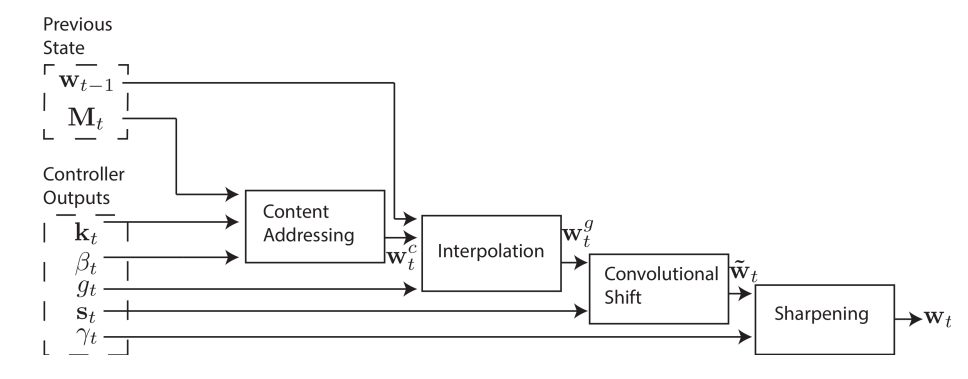
\includegraphics[scale=0.4]{images/weight_emission.png}
\end{center}

\begin{enumerate}
    \item First, each head produces a key vector and key strength factor which is used for content-based addressing, comparing each memory cell to the key vector to produce a weighting over the memory bank.
    \item Second, the content-based weighting is interpolated with the weight vector from the previous time step, essentially deciding how much of the old weighting to keep and how much to replace with the new content-based weighting.
    \item Third, the updated content-based weighting is rotationally shifted using a vector produced by each head; the purpose of the rotation is to allow the heads to incorporate location-based addressing into the weighting, enabling them to shift the weights over to the locations they want to focus on.
    \item Finally, the weighting is sharpened, widening the variance in the weights by amplifying large weights and decaying small ones, to account for the blurrying that occurred in the above steps. After this, the new vector vector is emitted by the heads.
\end{enumerate}

\subsubsection{Content-Based Addressing}
Generally speaking, content-based addressing is a way of retrieving information from storage in a way that depends on the content of the memory we want, rather than specific locations (a bit like the difference between a hash table, which allows one to easily lookup data by attributes about it, and an array, which allows one to easily lookup data based on its location in the array). The application of attention mechanisms to neural networks was loosely inspired by the human visual attention mechanism, which allows the eye to focus on certain regions of the visual field with high resolution, at the expense of the rest of the visual field; moreover the focal point and amount of focus are adjustable.
\newline \newline
As before we let $ M^t $ denote the ($ n \times m $) memory bank at time step $ t $. The process for emitting the weight vector begins by having each head produce a \textit{key vector}, $ k^t \in \mathbb{R}^m $, which essentially represents the content we want to search the memory bank for. We then construct a content-based weight vector, $ c^t $, by comparing each cell in the memory to the key vector (which represents the content we're searching for), using some similarity measure (usually cosine similarity) $ K: \mathbb{R}^m \times \mathbb{R}^m \rightarrow \mathbb{R}^+ $, which is then normalized:
$$ c^t = \text{softmax}\left( \begin{bmatrix} \beta^t K(k^t, M^t_i), 1 \leq i \leq n \end{bmatrix} \right) $$
where $ \beta^t \in \mathbb{R} $ is the \textit{key strength}, basically just an adjustable factor allowing us to amplify or attenuate the precision of the focus (higher values mean sharper focus).

\subsubsection{Location-Based Addressing}
Location-based addressing is the more common form of addressing used in standard computers, wherein data is referenced by its location in memory. Technically, content-based addressing is a stronger than location-based addressing (since we could supercede the latter into the former by including location as part of the content), but it's useful in practice to explicitly implement the two separately. At this stage in the weight emission pipeline, we've generated a content-based weight distribution $ c^t $ - to incorporate location into the distribution, we simply rotate $ c^t $ to shift the focus up or down to the locations (ie cell indices in $ M^t $) we want to focus on.
\newline \newline
First, we decide how much to update our existing weight distribution $ w^{t - 1} $ by the new content-based weight distribution. This is done by having each head first produce an \textit{interpolation gate} $ g^t \in (0, 1) $, which we use to update the weighting and yield a \textit{gated weighting} $ G^t $:
$$ G^t = g^t c^t + (1 - g^t) w^{t - 1} $$
\newline
Next, we perform the rotational shift by having each head produce a \textit{shift weighting} $ s^t $, which is just a normalized distribution of allowed integer shifts, with each scalar value representing how much to shift the corresponding index by. We thus perform the shift with a simple convolution followed by a re-normalization:
$$ w^t = \text{softmax}(G^t * s^t) \text{ where } * \text{ is the convolution operator: } (G^t * s^t)_i = \sum_{j = 0}^{n - 1} G^t_j s^t_{(i - j) \text{ mod } n} $$
Sometimes, the weights are sharpened to offset any blurriness that was probably imparted on the weight vector. This just means that the rift between values is enhanced, usually by raising each component to a power greater than one before passing through the softmax. This concludes the process of computing the weight $ w^t $, which is then emitted by each head and used in the read and write opertions as described in those sections.

\section{Hyperparameters}
The architecture detailed above lays out the prototypical version of the NTM, but there are many variations in the architecture one may use, depending on the problem. As with any model, there are several tunable hyperparameters, such as the size of the memory, the number of read and write heads, the range of allowed location shifts, etc. One major architectural decision is which neural network to use as the controller, since both feedforward and recurrent networks will work. RNNs can either augment or overcomplicate the model, especially LSTMs, which have their own sort of long-term memory built in.

\end{document}
